\documentclass[12pt,a4paper]{report}

\setcounter{section}{0}
\renewcommand{\thesection}{\arabic{section}}
\renewcommand{\thesubsection}{\thesection.\arabic{subsection}}
\renewcommand{\thesubsubsection}{\thesubsection.\arabic{subsubsection}}

\usepackage[utf8]{inputenc}
\usepackage{graphicx}
\usepackage{geometry}
\usepackage{setspace}
\usepackage{mathptmx}
\usepackage{caption}
\usepackage{float}
\usepackage{hanging}
\usepackage{hyperref}
\usepackage{booktabs}
\usepackage{longtable}
\usepackage{array}
\usepackage{enumitem}
\usepackage{fancyhdr}
\usepackage{titlesec}
\usepackage{parskip}

% Page geometry (guidelines: Top 1.5", Bottom 1.0", Left 2.0", Right 1.0")
\setlength{\headheight}{14.5pt}
\geometry{
  a4paper,
  top=1.5in,
  bottom=1.0in,
  left=1.0in,
  right=1.0in
}

\onehalfspacing
\setlength{\parskip}{6pt}

% Section heading fonts (Arial-like via sans-serif)
\titleformat{\section}{\sffamily\bfseries\fontsize{16}{20}\selectfont}{\thesection.}{0.5em}{}
\titleformat{\subsection}{\sffamily\bfseries\fontsize{14}{18}\selectfont}{\thesubsection}{0.5em}{}
\titleformat{\subsubsection}{\sffamily\bfseries\itshape\fontsize{13}{17}\selectfont}{\thesubsubsection}{0.5em}{}

\pagestyle{fancy}
\fancyhf{}
\fancyhead[RO]{Mahir on Call: Advanced Elucidation Support in Local Language}
\fancyhead[RE]{\leftmark}
\fancyfoot[R]{\thepage}
\renewcommand{\headrulewidth}{0.4pt}

\hypersetup{
  colorlinks=true,
  linkcolor=black,
  urlcolor=blue,
  citecolor=black
}

\begin{document}

% =====================  TITLE PAGE  ==================================
\begin{titlepage}
  \thispagestyle{empty}
  \centering
  {\setstretch{1.1}
    \fontsize{26}{32}\selectfont\bfseries Mahir on Call\\[0.4cm]
    \fontsize{20}{26}\selectfont\bfseries Advanced Elucidation Support in Local Language
  }\\[2.0cm]

  {\large Session 2022--2026}\\[0.5cm]
  {\large \textbf{Supervised by}}\\
  {\large Muhammad Umer Haroon}\\[0.4cm]
  {\large \textbf{Co-supervised by}}\\
  {\large Shahzeb Khan}\\[2.0cm]

  \vfill
  \includegraphics[width=0.28\textwidth]{universityLogo.png}\\[1.2cm]

  {\large Department of Computer Science}\\[0.4cm]
  {\Large National University of Computer and Emerging Sciences}\\[0.3cm]
  {\Large Peshawar, Pakistan}
\end{titlepage}

\pagenumbering{roman}
\setcounter{page}{1}

% =====================  STUDENT'S DECLARATION  =======================
\newpage
\thispagestyle{plain}
\begin{center}
  {\Large \textbf{Student's Declaration}}\\[1cm]
\end{center}

\noindent We declare that this project titled \textit{Mahir on Call: Advanced
Elucidation Support in Local Language}, submitted as requirement for the award
of degree of Bachelors in Computer Science, does not contain any material
previously submitted for a degree in any university; and that to the best of
our knowledge, it does not contain any materials previously published or
written by another person except where due reference is made in the text.\\[0.5cm]

\noindent We understand that the management of the Department of Computer
Science, National University of Computer and Emerging Sciences, has a
zero-tolerance policy towards plagiarism. Therefore, we, as authors of the
above-mentioned thesis, solemnly declare that no portion of our thesis has
been plagiarized, and any material used in the thesis from other sources is
properly referenced.\\[0.5cm]

\noindent We further understand that if we are found guilty of any form of
plagiarism in the thesis work even after graduation, the University reserves
the right to revoke our BS degree.\\[1.2cm]

\begin{tabular}{p{7cm} p{6cm}}
  Uzair Ahmad      & Signature: \hrulefill \\[1cm]
  Arsalan Mateen   & Signature: \hrulefill \\[1cm]
  Muhammad Sohaib  & Signature: \hrulefill \\
\end{tabular}

\vfill
\begin{flushright}
  \begin{tabular}{l}
    \hrulefill \\
    Verified by Plagiarism Cell Officer \\
    Dated: \underline{\hspace{4cm}} \\
  \end{tabular}
\end{flushright}

% =====================  CERTIFICATE OF APPROVAL  =====================
\newpage
\thispagestyle{plain}
\begin{center}
  {\Large \textbf{Certificate of Approval}}\\[0.8cm]
  \includegraphics[width=0.25\textwidth]{universityLogo.png}\\[0.8cm]
\end{center}

\noindent The Department of Computer Science, National University of Computer
and Emerging Sciences, accepts this thesis titled \textit{Mahir on Call:
Advanced Elucidation Support in Local Language}, submitted by Uzair Ahmad,
Arsalan Mateen, and Muhammad Sohaib, in its current form, as fulfilling the
dissertation requirements for the award of Bachelors Degree in Computer
Science.\\[1.5cm]

\begin{center}
  \makebox[0.55\linewidth]{\hrulefill}\\
  Prof. Muhammad Umer Haroon\\
  FYP Supervisor\\
  National University of Computer and Emerging Sciences, Peshawar\\[1.5cm]

  \makebox[0.55\linewidth]{\hrulefill}\\
  Riaz Nawab\\
  FYP Coordinator\\
  National University of Computer and Emerging Sciences, Peshawar\\[1.5cm]

  \makebox[0.55\linewidth]{\hrulefill}\\
  Dr. Qasim Jaan\\
  HoD, Department of Computer Science\\
  National University of Computer and Emerging Sciences, Peshawar
\end{center}

% =====================  ACKNOWLEDGMENT  ==============================
\newpage
\thispagestyle{plain}
\begin{center}
  {\Large \textbf{Acknowledgment}}\\[1cm]
\end{center}

\noindent We owe our first thanks to our supervisor, \textbf{Muhammad Umer
Haroon}, who guided us steadily from the very first week of the project. He
pushed us to think harder when we tried to take shortcuts and was generous
with his time whenever we got stuck. The shape this report has now owes a lot
to his early steering.\\[0.5cm]

\noindent We are also sincerely thankful to our co-supervisor, \textbf{Shahzeb
Khan}, who stepped in during some of the harder phases of the build. His
advice was practical, and he had a way of pulling us back from
over-engineering when we were tempted to chase nice-to-have features instead
of finishing the core.\\[0.5cm]

\noindent We extend our appreciation to the administration and staff of
\textbf{FAST Peshawar}, who answered our questions about the kinds of queries
they handle every day, gave us the domain knowledge that informed the system
design, and let us trial the application in a real setting.\\[0.5cm]

\noindent Finally, we are grateful to our families, friends, and peers for
their moral support and encouragement during this journey.\\[1.2cm]

\begin{flushright}
  Uzair Ahmad\\
  Arsalan Mateen\\
  Muhammad Sohaib
\end{flushright}

% =====================  ABSTRACT  ====================================
\newpage
\thispagestyle{plain}
\begin{center}
  {\Large \textbf{Abstract}}\\[1cm]
\end{center}

\noindent Every admission season, the front desk of FAST-NUCES Peshawar is
hit with a wave of queries that arrive faster than the staff can answer them.
Most of the questions are repetitive, and most of them come in Urdu rather
than English. Yet the digital channels through which a university speaks to
its applicants, such as its website, its forms, and its email, are almost
always English first. This report presents \textit{Mahir on Call}, a real
time Urdu voice AI web application built for the front desk of FAST-NUCES
Peshawar. A visitor can speak a question in Urdu inside any modern browser.
The system writes the speech down, looks up the answer in a curated knowledge
base, generates a clear reply, speaks it back, and shows a written transcript
on screen at the same time. The pipeline combines a multilingual speech
recognition stage, a retrieval augmented language model that stays grounded
in official documents, and a neural text to speech stage for natural Urdu
audio output. A moderator interface allows administrative staff to handle
queries that fall outside the system's knowledge. Evaluation shows the
system reduces routine response time and improves accessibility for Urdu
speaking applicants who are otherwise underserved by English first digital
channels.

% =====================  EXECUTIVE SUMMARY  ===========================
\newpage
\thispagestyle{plain}
\begin{center}
  {\Large \textbf{Executive Summary}}\\[1cm]
\end{center}

\noindent \textit{Mahir on Call: Advanced Elucidation Support in Local
Language} is a Final Year Project developed by students of the Department of
Computer Science, FAST-NUCES Peshawar, for the academic session 2022 to
2026. The project tackles a real operational problem in university admission
offices. During the admission season, the volume of voice and email queries
is far higher than what the staff can comfortably handle in good time and in
the language most applicants are most fluent in.\\[0.3cm]

\noindent The system is a browser based voice AI application that any
visitor can open directly from the university website. There is nothing to
install. Once the page loads, the user can start a voice conversation in
Urdu with the assistant. The assistant listens, writes down the speech, and
understands the query through a pipeline that combines automatic speech
recognition, natural language understanding, and a domain specific retrieval
augmented generation engine. A text to speech module then speaks the
generated answer back in Urdu, while the chat panel shows a live transcript
on screen for users who prefer to read.\\[0.3cm]

\noindent Key features include real time Urdu voice interaction, live
transcription, multi turn conversation memory, audio playback that the user
can interrupt at any time, and a knowledge base built from official
FAST Peshawar admission documents. A secure admin panel allows authorised
staff to update the knowledge base without touching code.\\[0.3cm]

\noindent The project is scoped specifically to FAST Peshawar admission
queries. It demonstrates that a domain specific conversational AI in a local
language is feasible inside the time and budget of a Final Year Project, and
that the same architecture can serve other Pakistani universities facing the
same operational pressure.

% =====================  TABLE OF CONTENTS  ===========================
\newpage
\tableofcontents

% =====================  BODY  ========================================
\newpage
\pagenumbering{arabic}
\setcounter{page}{1}

% ============================================================
% 1. INTRODUCTION
% ============================================================
\newpage
\section{Introduction}

Conversational AI has moved from research labs into everyday products at a
remarkable pace. Even so, its adoption in regional language and domain
specific settings is still limited. The higher education sector in Pakistan
sees this gap clearly. During the admission season, students and parents who
mostly speak Urdu flood the university helplines with questions that are
repetitive, time sensitive, and very similar in nature. Staff capacity is
fixed, and the resulting delays often translate into a poor experience for
the applicant and a lost hour for the admin team.

Mahir on Call (which means \textit{Expert on Call}) is a real time voice AI
web application built for the National University of Computer and Emerging
Sciences, FAST. It allows any visitor to the university website to speak a
question in Urdu and get an instant spoken reply. There is no email to
send, no menu tree to follow, and no operator to wait for. The interface
runs in any modern browser, so even a low end phone with a working data
connection is enough to use it.

A live transcript is displayed alongside the audio reply for users who are
deaf or hard of hearing, and for users who simply prefer to read. The
overall flow is illustrated in Figure~\ref{fig:architecture}.

\begin{figure}[H]
  \centering
  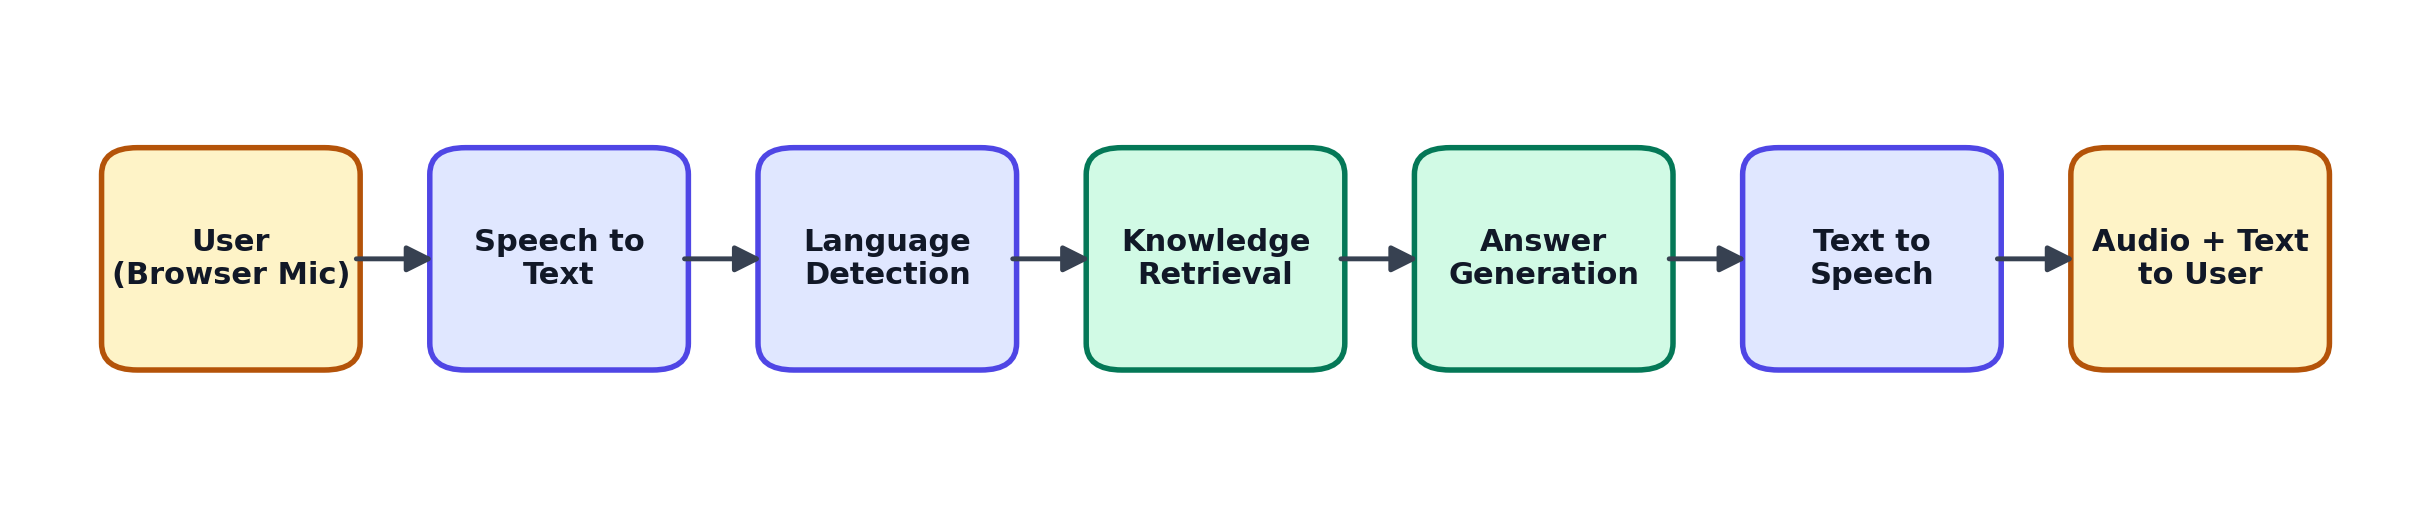
\includegraphics[width=0.95\textwidth]{figures/fig1_pipeline_architecture.png}
  \caption{High level pipeline architecture of Mahir on Call.}
  \label{fig:architecture}
\end{figure}

% ============================================================
% 2. RESEARCH ON EXISTING PRODUCTS
% ============================================================
\newpage
\section{Research on Existing Products}

Before we built anything, we surveyed the conversational AI products that
already exist for higher education and customer support. The aim was to
understand what these systems do well, where they fall short for Urdu
speakers, and what those gaps mean for our own design.

\subsection{General Purpose Voice Assistants}

Products such as Amazon Alexa, Google Assistant, and Apple Siri are built
for broad consumer use. They support many languages on paper, but they do
not have deep knowledge about specific institutions, and they cannot be
customised to answer university specific queries without a serious
engineering investment. They also do not natively support Urdu in a way
that is tuned for Pakistani phonology, vocabulary, or the kind of code
switching most of our users actually speak. In a setting where the right
answer to a question about a fee deadline must be exactly right, a closed
assistant that we cannot constrain to a known knowledge base is not a good
fit. A confident but wrong answer is worse than no answer at all.

\subsection{University Chatbot Platforms}

Several universities around the world have rolled out text based chatbots
for student services. A well known example is a chatbot deployed at
Georgia Tech that used an enterprise NLP stack to answer frequently asked
questions on online course forums. This kind of system shows that a domain
specific chatbot can be very accurate when its scope is well defined and
its training material is curated. However, these systems are mostly
English only and text only. They do not serve users who would rather speak
than type, and they do not serve users whose first language is not
English.

\subsection{Customer Service Voice AI}

Commercial platforms such as Dialogflow CX from Google, Amazon Lex, and
the Azure Bot Service from Microsoft offer full stack infrastructure for
voice enabled chatbots. They are powerful, but they need a lot of
configuration, their hosted licensing costs grow with usage, and none of
them ships with an Urdu acoustic model that is tuned for Pakistani speech.
Wiring a knowledge base grounded retrieval pipeline into them is a
substantial piece of work in its own right. An open source self hosted
alternative removes the recurring licensing cost, but its dialogue
manager wants a lot of labelled training data and does not sit naturally
with the modern language model based response generation that gives our
system its flexibility.

% ============================================================
% 3. PROJECT VISION
% ============================================================
\newpage
\section{Project Vision}

\subsection{Problem Statement}

During the annual admission season, the administrative offices of
FAST-NUCES Peshawar receive hundreds of emails and phone calls every day
from prospective students and their parents. The questions cover a small
set of topics that come up again and again: eligibility criteria, the
NU-Test, application procedures, fee structures, scholarship policies, and
hostel availability. The volume of queries goes well beyond what the staff
can answer in good time. The result is delayed replies, frustrated
applicants, and a team that spends most of the day on routine lookups
instead of the cases that actually need their judgement. A meaningful
portion of the applicant pool is more comfortable in Urdu than in English,
and the existing English first digital channels make it harder for that
group to access timely information.

\subsection{Business Opportunity}

A round the clock Urdu voice AI service embedded in the university website
removes the dependency on human operators for routine repetitive queries.
It cuts operational costs, improves applicant satisfaction, and positions
FAST Peshawar as a technology forward institution that takes its Urdu
speaking applicants seriously. The same architecture can be extended to
other FAST campuses by swapping in a new knowledge base, and in the
longer term it can be offered to other Pakistani universities facing the
same operational pressure.

\subsection{Objectives}

\begin{itemize}
  \item Build a real time voice AI web application that runs in any modern
        browser without an installer.
  \item Support Urdu language voice input and output, since this is the
        language most of the target audience is most comfortable in.
  \item Provide instant accurate answers to admission related queries by
        grounding every reply in a retrieval based knowledge base built
        from official FAST Peshawar documents.
  \item Display a live transcript of the conversation for users who are
        deaf, hard of hearing, or who simply prefer to read.
  \item Keep the average end to end response latency under five seconds for
        typical queries so the conversation feels natural.
\end{itemize}

\newpage
\subsection{Constraints}

\begin{itemize}
  \item The assistant can only answer queries that are inside its knowledge
        base. Anything outside that scope is escalated to the moderator.
  \item Real time voice processing needs a stable broadband connection.
        Performance degrades on slow networks.
  \item The accuracy of the assistant is bounded by the quality and
        coverage of the knowledge base. Outdated content leads to
        outdated replies, so the knowledge base must be reviewed before
        each admission season.
  \item Browser microphone capture is not equally well supported across
        all browsers. Chrome and Edge give the best experience.
\end{itemize}

% ============================================================
% 4. SOFTWARE REQUIREMENT SPECIFICATIONS
% ============================================================
\newpage
\section{Software Requirement Specifications}

\subsection{List of Features}

\begin{itemize}
  \item \textbf{Real time Voice Conversation}:
        Users can speak to the assistant and receive spoken replies in
        Urdu.
  \item \textbf{Live Transcription}:
        The full conversation is transcribed and shown on screen as it
        unfolds.
  \item \textbf{Urdu Language Support}:
        The system runs in Urdu by default with an English fallback.
  \item \textbf{Knowledge Base}:
        Replies are generated from a curated retrieval based knowledge
        base of official FAST Peshawar documents.
  \item \textbf{Interruptible Playback}:
        The user can stop a playing reply at any time and start a new
        query without losing the conversation history.
  \item \textbf{Conversation Memory}:
        The last few exchanges are kept in context so follow up questions
        can be resolved correctly.
  \item \textbf{Graceful Fallback}:
        When the assistant cannot answer with confidence, the user is
        offered a route to the moderator instead of a guess.
  \item \textbf{Admin Panel}:
        Authorised staff can review the current knowledge base and upload
        new content without touching the code.
\end{itemize}

\subsection{Functional Requirements}

\begin{longtable}{p{2cm} p{4cm} p{8.5cm}}
  \toprule
  \textbf{ID} & \textbf{Feature}         & \textbf{Requirement} \\
  \midrule
  \endhead
  FR-01 & Voice Input           & The system shall capture microphone audio from the browser and pass it to the speech recognition module. \\[4pt]
  FR-02 & Speech to Text        & The system shall transcribe spoken Urdu and English with a Word Error Rate of 25\% or below on a reference test set. \\[4pt]
  FR-03 & Language Detection    & The system shall detect whether the input is Urdu or English and route the query through the right processing path. \\[4pt]
  FR-04 & Query Understanding   & The system shall embed the transcribed query and retrieve the most relevant context chunks from the knowledge base. \\[4pt]
  FR-05 & Response Generation   & The system shall generate a clear and accurate response that stays inside the retrieved context. \\[4pt]
  FR-06 & Text to Speech        & The system shall convert the generated text into natural Urdu or English audio and play it back in the browser. \\[4pt]
  FR-07 & Live Transcript       & The system shall display the running conversation as text in real time. \\[4pt]
  FR-08 & Conversation Memory   & The system shall keep the last three exchanges of a session and pass them as history with each new query. \\[4pt]
  FR-09 & Interrupt Playback    & The system shall let the user stop a playing reply at any time and return the interface to idle. \\[4pt]
  FR-10 & Moderator Access      & The system shall route any query that falls outside the knowledge base to a designated moderator. \\[4pt]
  FR-11 & Admin Authentication  & The admin panel shall require valid credentials before any knowledge base management is allowed. \\[4pt]
  FR-12 & Knowledge Ingestion   & The admin panel shall accept plain text files, split them into overlapping chunks, embed the chunks, and store them with stable identifiers so re-uploads do not create duplicates. \\[4pt]
  \bottomrule
\end{longtable}

\newpage
\subsection{Non-Functional Requirements}

\begin{longtable}{p{2cm} p{3.5cm} p{9cm}}
  \toprule
  \textbf{ID} & \textbf{Category}    & \textbf{Requirement} \\
  \midrule
  \endhead
  NFR-01 & Performance          & End to end response latency shall be under five seconds for 90\% of queries on a connection of 10 Mbps or above. \\[4pt]
  NFR-02 & Accuracy             & The system shall return accurate in scope replies for at least 80\% of queries drawn from the evaluation test set. \\[4pt]
  NFR-03 & Availability         & The system shall target 99\% uptime during the admission season window. \\[4pt]
  NFR-04 & Scalability          & The system shall handle at least 20 concurrent voice sessions without noticeable degradation. \\[4pt]
  NFR-05 & Security             & All data in transit shall be encrypted using TLS 1.2 or above. No personally identifiable information shall be stored beyond the session. Configuration secrets shall be kept outside the source repository and loaded at runtime from a protected location on the deployment host. \\[4pt]
  NFR-06 & Usability            & A user with no technical background shall be able to start a voice conversation within 30 seconds of reaching the page. \\[4pt]
  NFR-07 & Accessibility        & The live transcript shall meet WCAG 2.1 Level AA contrast and text size guidelines. \\[4pt]
  NFR-08 & Maintainability      & Authorised non technical staff shall be able to update the knowledge base through the admin panel without access to the codebase. \\[4pt]
  \bottomrule
\end{longtable}

% ============================================================
% 5. ITERATION PLAN
% ============================================================
\newpage
\section{Iteration Plan}

The project was developed in three iterations. Each iteration was meant to
leave us with something we could actually run and demonstrate, even if it
was rough around the edges. The reason for breaking the work up this way
was simple. The riskiest parts of the project were Urdu speech
recognition that worked on Pakistani accents, and a language model that
would not invent facts about admission deadlines. We needed to validate
those parts early, before we had committed to a full feature list.

\subsection{Iteration 1: Voice Pipeline}

The first iteration was about wiring up the end to end voice pipeline and
checking that each chosen technology was good enough to keep. The
deliverable was a working prototype that could take a spoken query, write
it down, generate a reply from a small starter knowledge base, and return
the reply as synthesised audio.

\subsubsection{Use Case Diagram}

Figure~\ref{fig:usecase} shows the primary use cases of the system. It
involves two actors: the User (a prospective student or parent visiting
the website) and the Administrator (university staff with access to the
admin panel and to the moderator queue).

\begin{figure}[H]
  \centering
  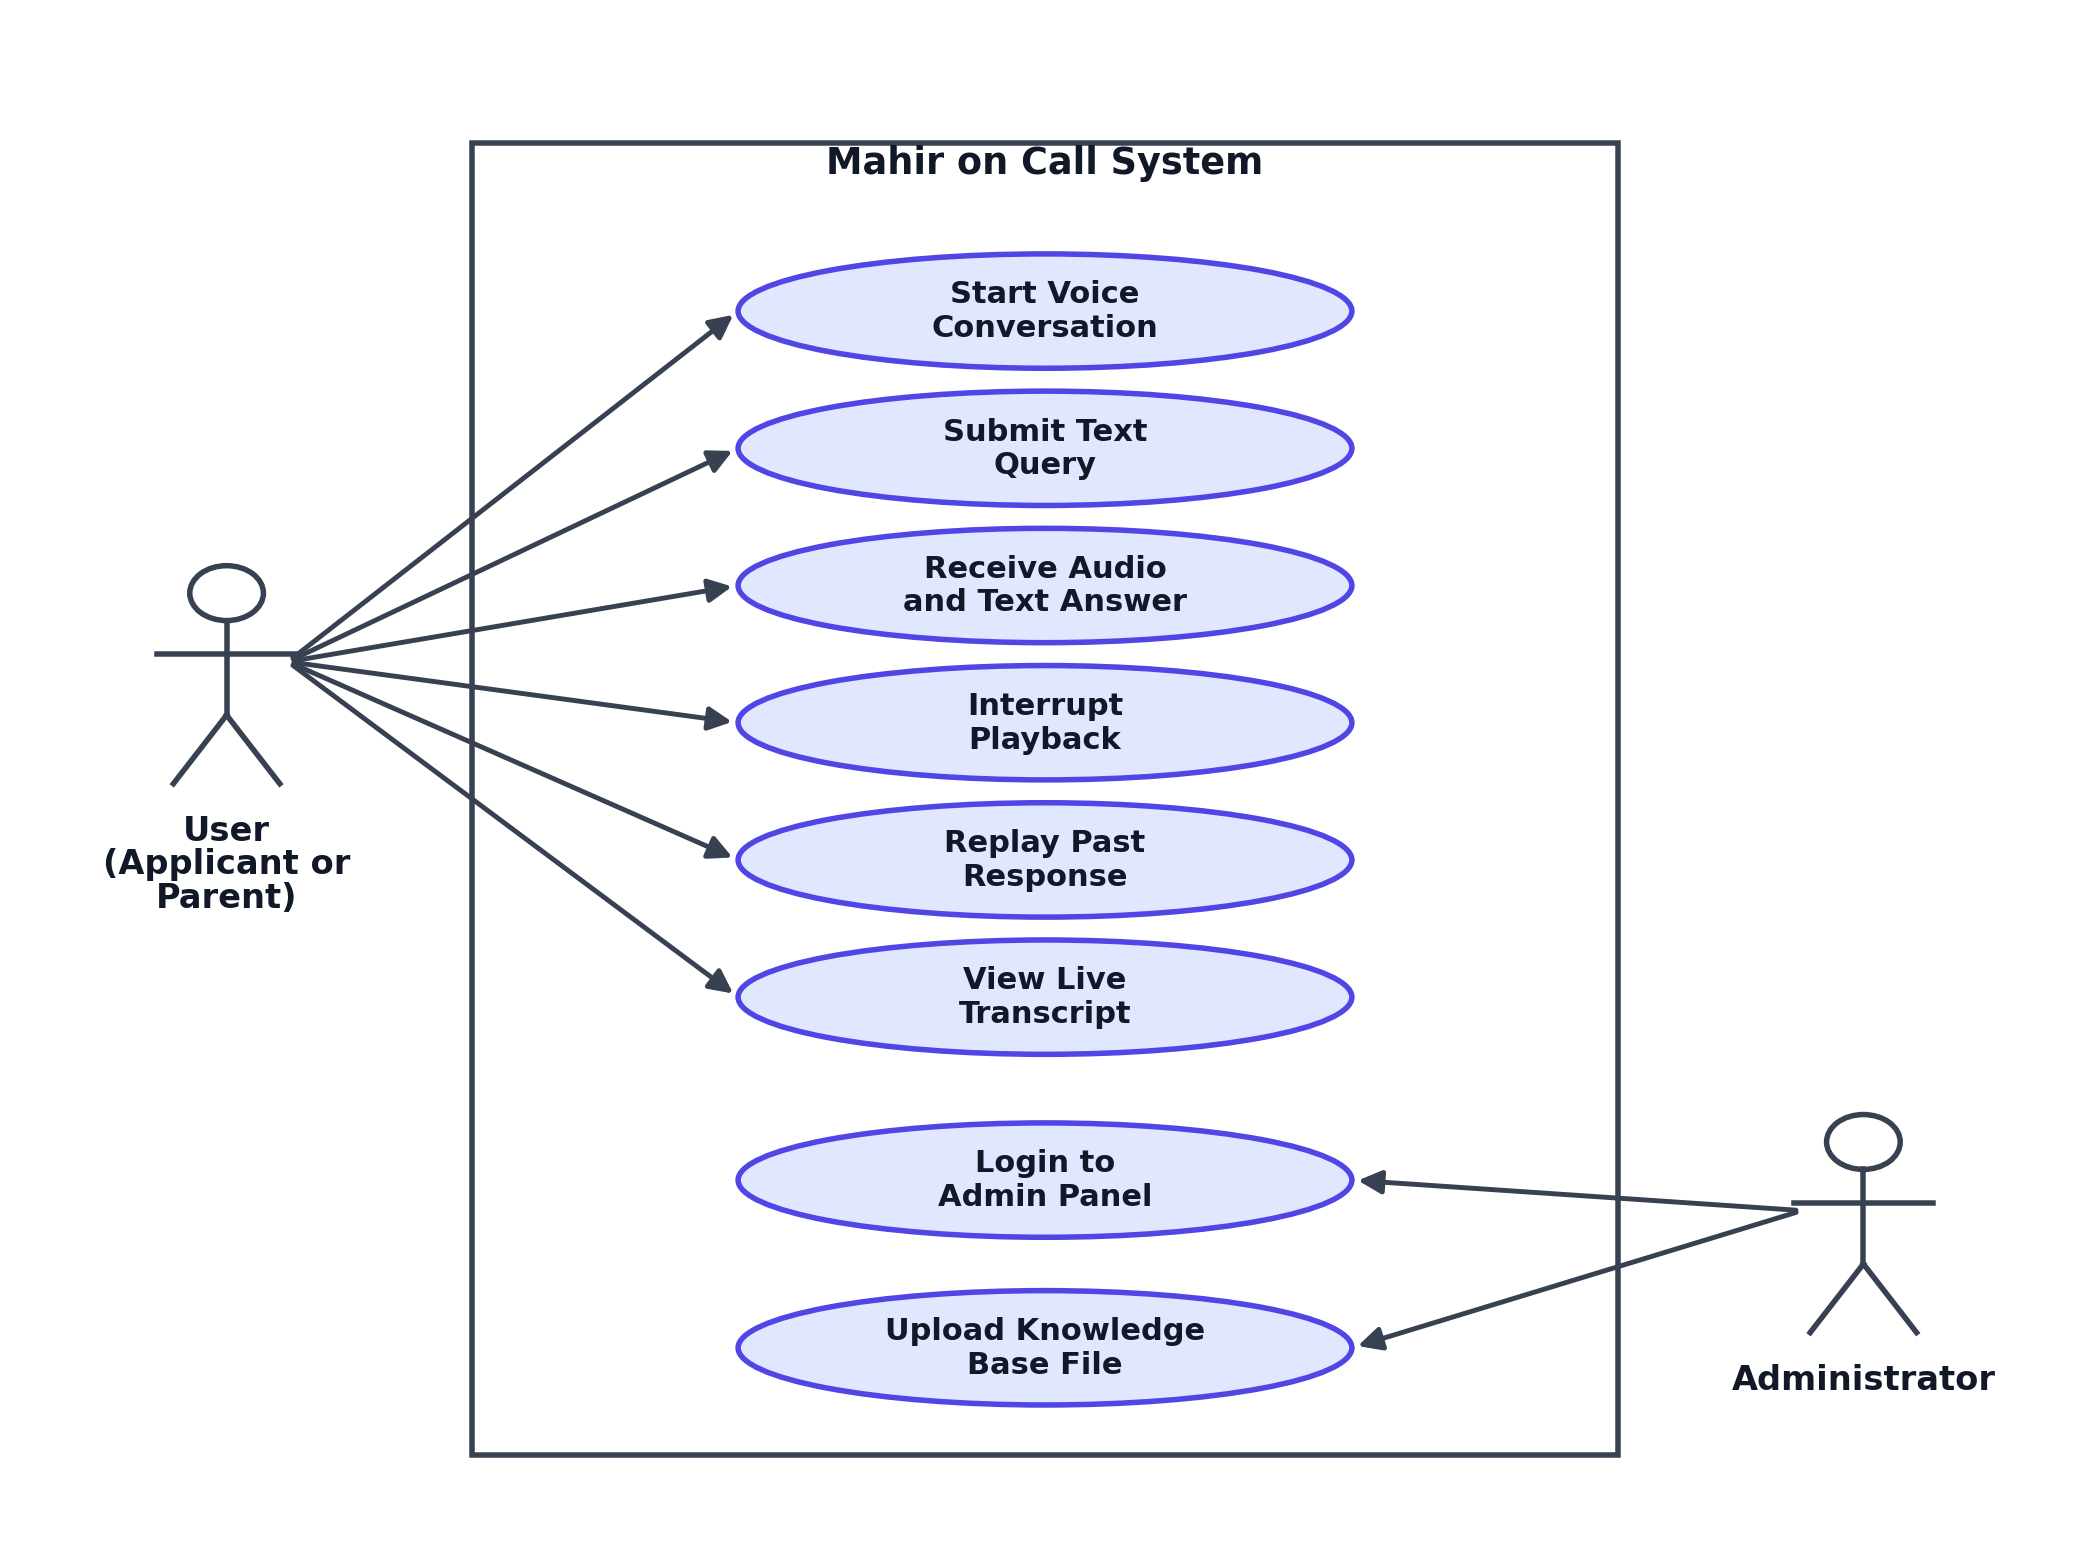
\includegraphics[width=0.85\textwidth]{figures/fig2_use_case_diagram.png}
  \caption{Use case diagram for Mahir on Call.}
  \label{fig:usecase}
\end{figure}

\subsubsection{Use Case Descriptions}

\begin{itemize}
  \item \textbf{Start Voice Conversation}:
        The user clicks the microphone button on the page. The browser
        asks for microphone permission and, once granted, starts
        capturing audio.
  \item \textbf{Submit Text Query}:
        The user types a question into the chat widget. The query is sent
        directly to the backend and skips the speech recognition stage.
  \item \textbf{Receive Audio and Text Answer}:
        The system returns the transcript of the user query, the text of
        the generated answer, and an audio version of the answer.
  \item \textbf{Interrupt Playback}:
        While audio is playing, the user can press the microphone button
        to stop it. Playback halts and the interface returns to idle.
  \item \textbf{Replay Past Response}:
        The user can press the speaker button on any earlier bubble to
        play the audio again on demand.
  \item \textbf{View Live Transcript}:
        During and after each exchange, the user sees the conversation
        transcript in text on screen.
  \item \textbf{Login to Admin Panel}:
        An authenticated administrator opens the admin panel using stored
        credentials.
  \item \textbf{Upload Knowledge Base File}:
        The administrator uploads a plain text file. The system splits
        it, embeds the chunks, and stores them with stable identifiers,
        so re-uploading the same file does not create duplicates.
\end{itemize}

\subsubsection{Voice Query Flow}

The activity diagram in Figure~\ref{fig:activity} shows the typical flow
of a voice query through the system. The user records audio in the
browser. The frontend sends it to the backend. The backend writes the
audio down and detects the language. The flow then branches between an
Urdu prompt and an English prompt, after which the two branches rejoin
for the retrieval, generation, and synthesis stages, and finally play
back to the user.

\begin{figure}[H]
  \centering
  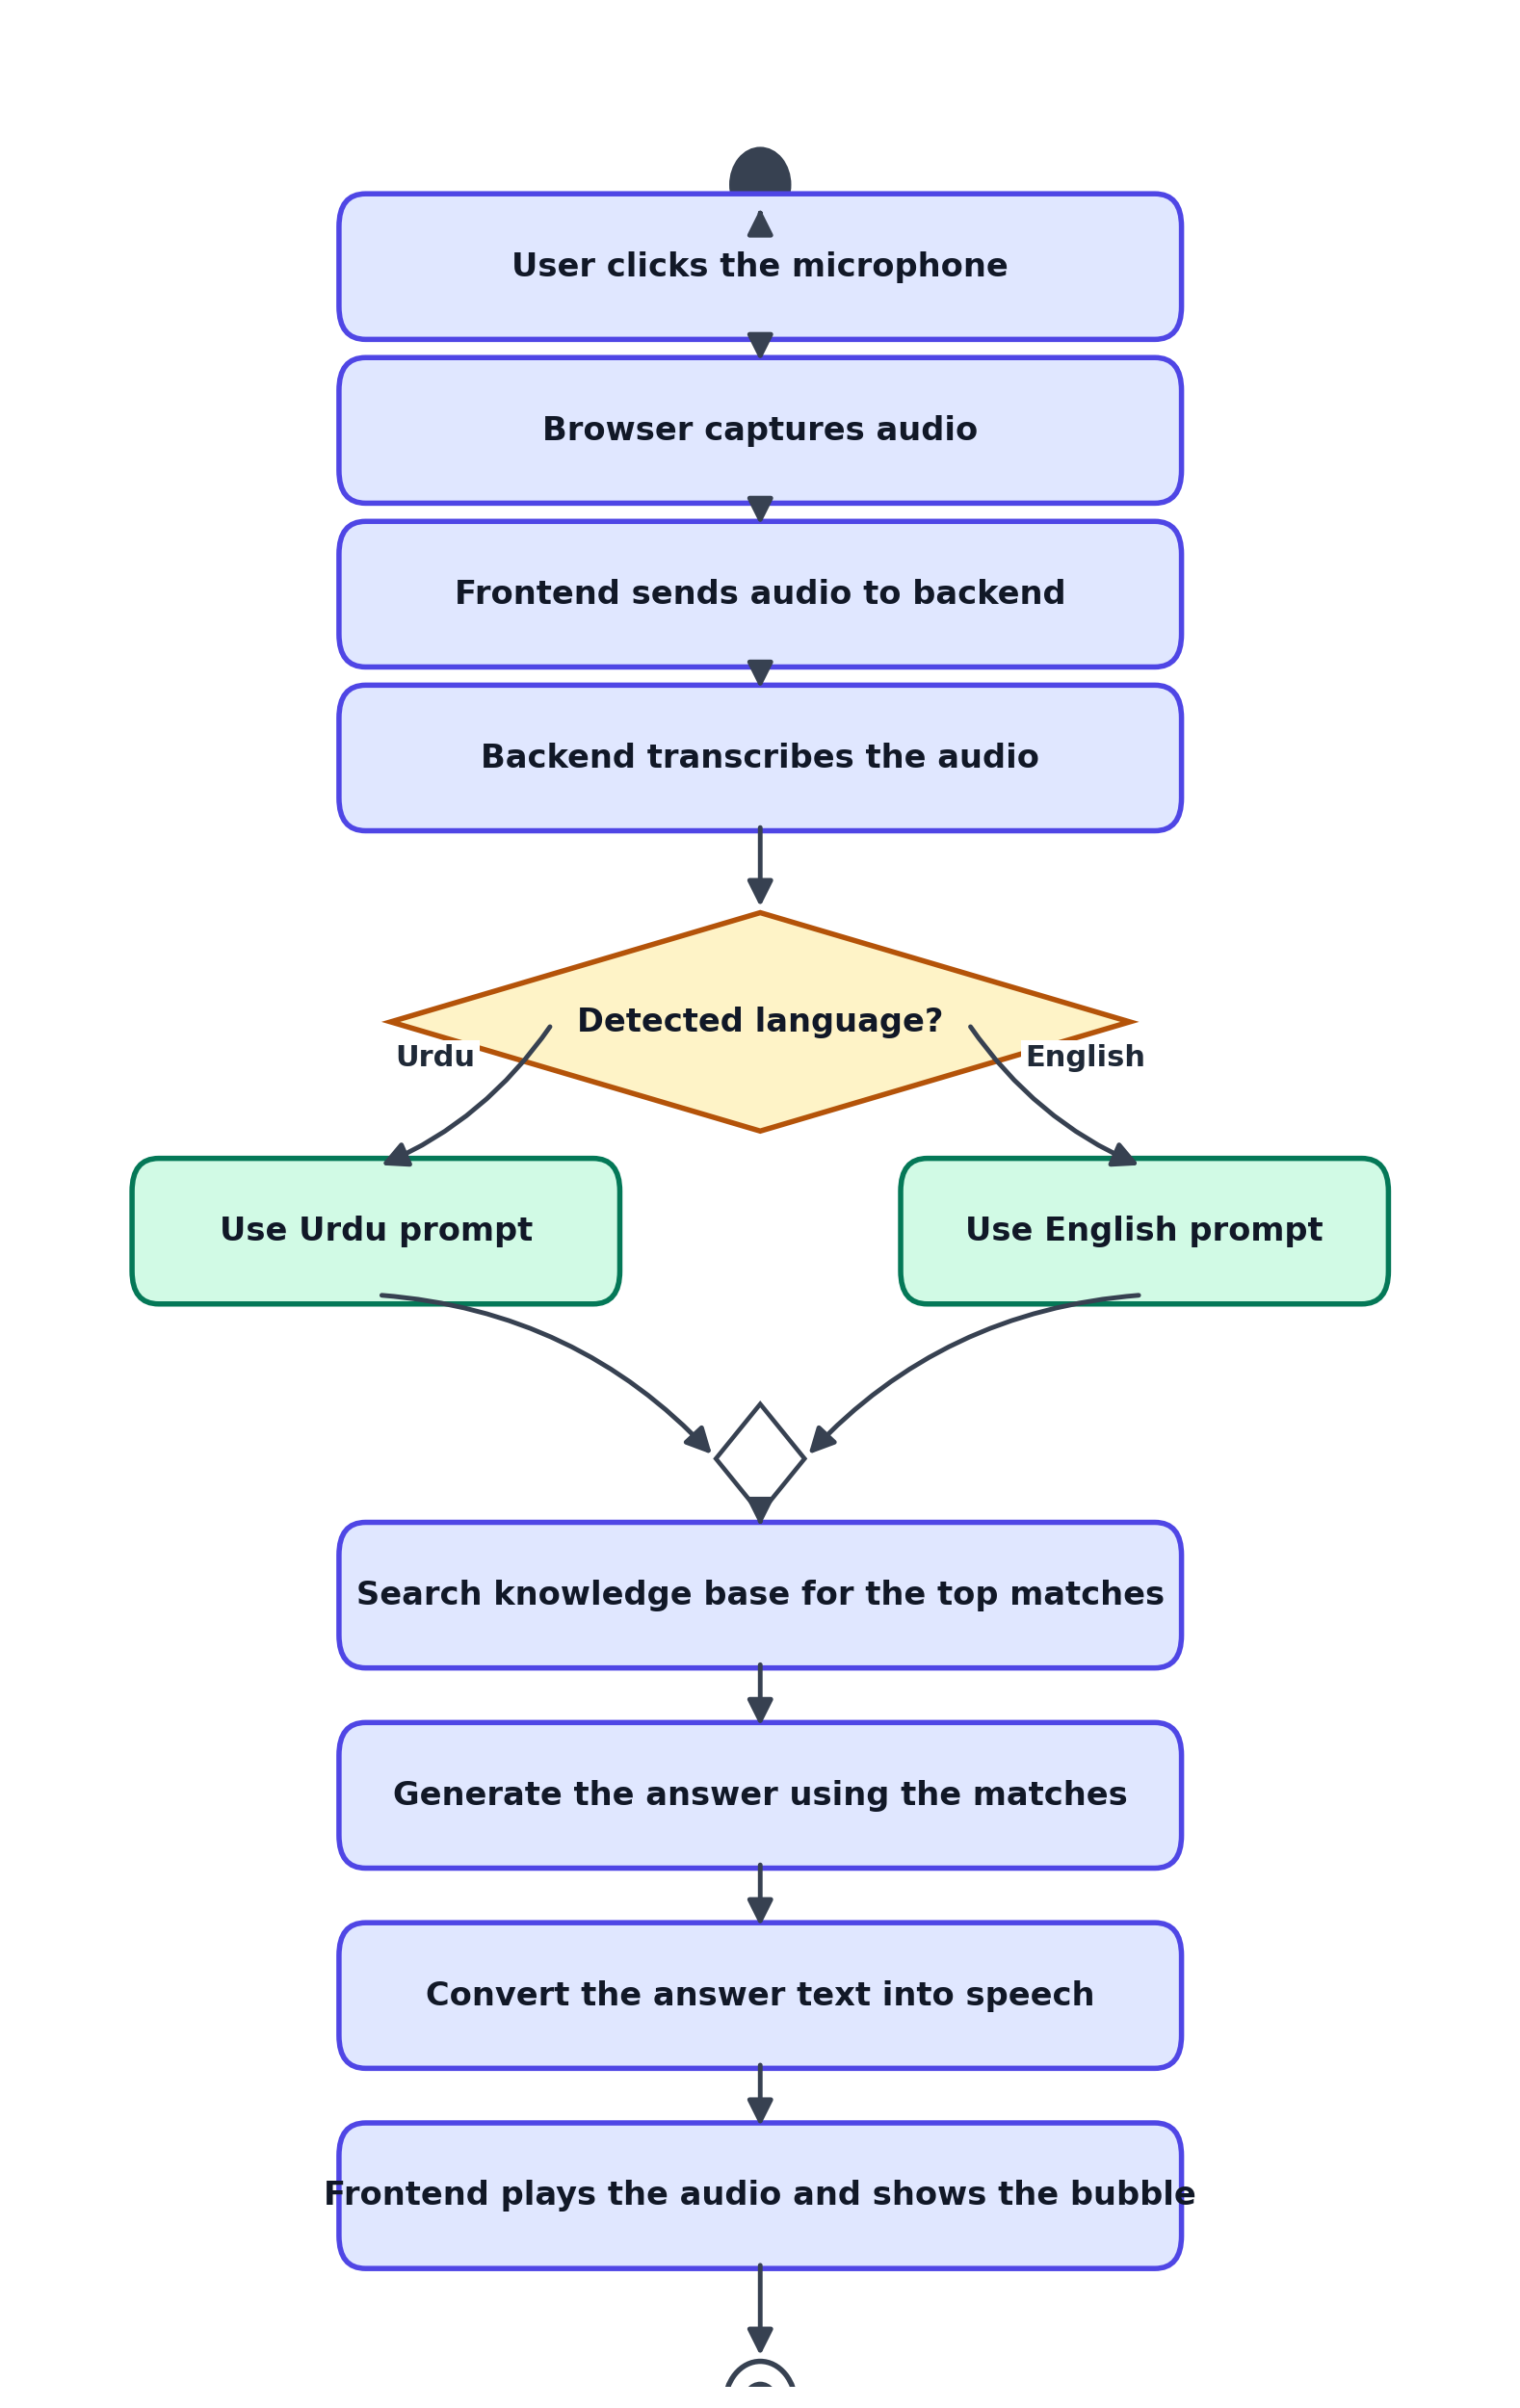
\includegraphics[width=0.65\textwidth]{figures/fig3_activity_diagram.png}
  \caption{Activity diagram for a voice query.}
  \label{fig:activity}
\end{figure}

\newpage
\subsection{Iteration 2: Knowledge Base}

The second iteration is where the knowledge base went from \textit{good
enough to demo} to something we could actually rely on, and where the
retrieval layer was tuned for the right tone of voice. The single file
knowledge base from the first iteration was scrapped in favour of a per
category structure. Each domain topic is now stored as its own source
file with its own chunk set and metadata. This had two useful side
effects. The admin panel can now show per source statistics. The system
prompt could be tuned for warm, context aware replies rather than the
terse one liners we were getting before.

The reply prompt went through a substantial rewrite during this
iteration. The first draft was technically accurate but came back with
answers that felt curt and that did not point users toward related
resources when the literal answer was \textit{no}. The revised prompt
asks the model to take a graduated approach: give a complete answer
when the knowledge base has one, give partial information with an honest
acknowledgement of what is missing when only some of the answer is
available, suggest a website link or a contact channel only when it
appears in the retrieved context and is genuinely relevant, and refer the
user to the moderator only when the question genuinely needs a human.

A small text to speech preprocessing step was also added during this
iteration. URLs are replaced by the spoken word \textit{Link} so they do
not get pronounced one letter at a time. A hardcoded dictionary maps
known institutional abbreviations to forms that sound more natural. Any
remaining four or more character all caps token is converted to title
case as a final fallback, so unfamiliar acronyms still read smoothly.

\subsection{Iteration 3: Refinement}

The third iteration was about polishing the user experience and getting
the system ready to be handed over. The chat widget was rebuilt as a
WhatsApp style panel that supports both voice and text input, with
timestamped bubbles and on demand speaker buttons in place of automatic
playback. Multi turn conversation memory was added by passing the last
three exchanges as history alongside each new query, so follow up
questions are resolved correctly. The interrupt feature was finished, so
a user can stop a playing reply without waiting for it to end. The admin
panel was built as a separate route inside the existing frontend, with a
login gate, a status table of the current knowledge base, and a drag and
drop upload zone.

\subsubsection{Live Transcription}

A streaming connection is used to push each recognised word from the
speech stage back to the browser as soon as it is available. The chat
panel updates word by word, which gives the user immediate feedback that
the system is hearing them and reduces the perceived latency of the
overall reply.

\subsubsection{Frontend State Machine}

The voice recorder logic in the frontend is implemented as a small state
machine. Figure~\ref{fig:state} shows the five states and the events
that move the interface between them. The states are \textit{idle},
\textit{listening}, \textit{processing}, \textit{responding}, and
\textit{error}. The diagram makes the corner cases explicit, including
the user dismissing an error, a microphone permission denial during
listening, and the user interrupting playback to start a new query.

\begin{figure}[H]
  \centering
  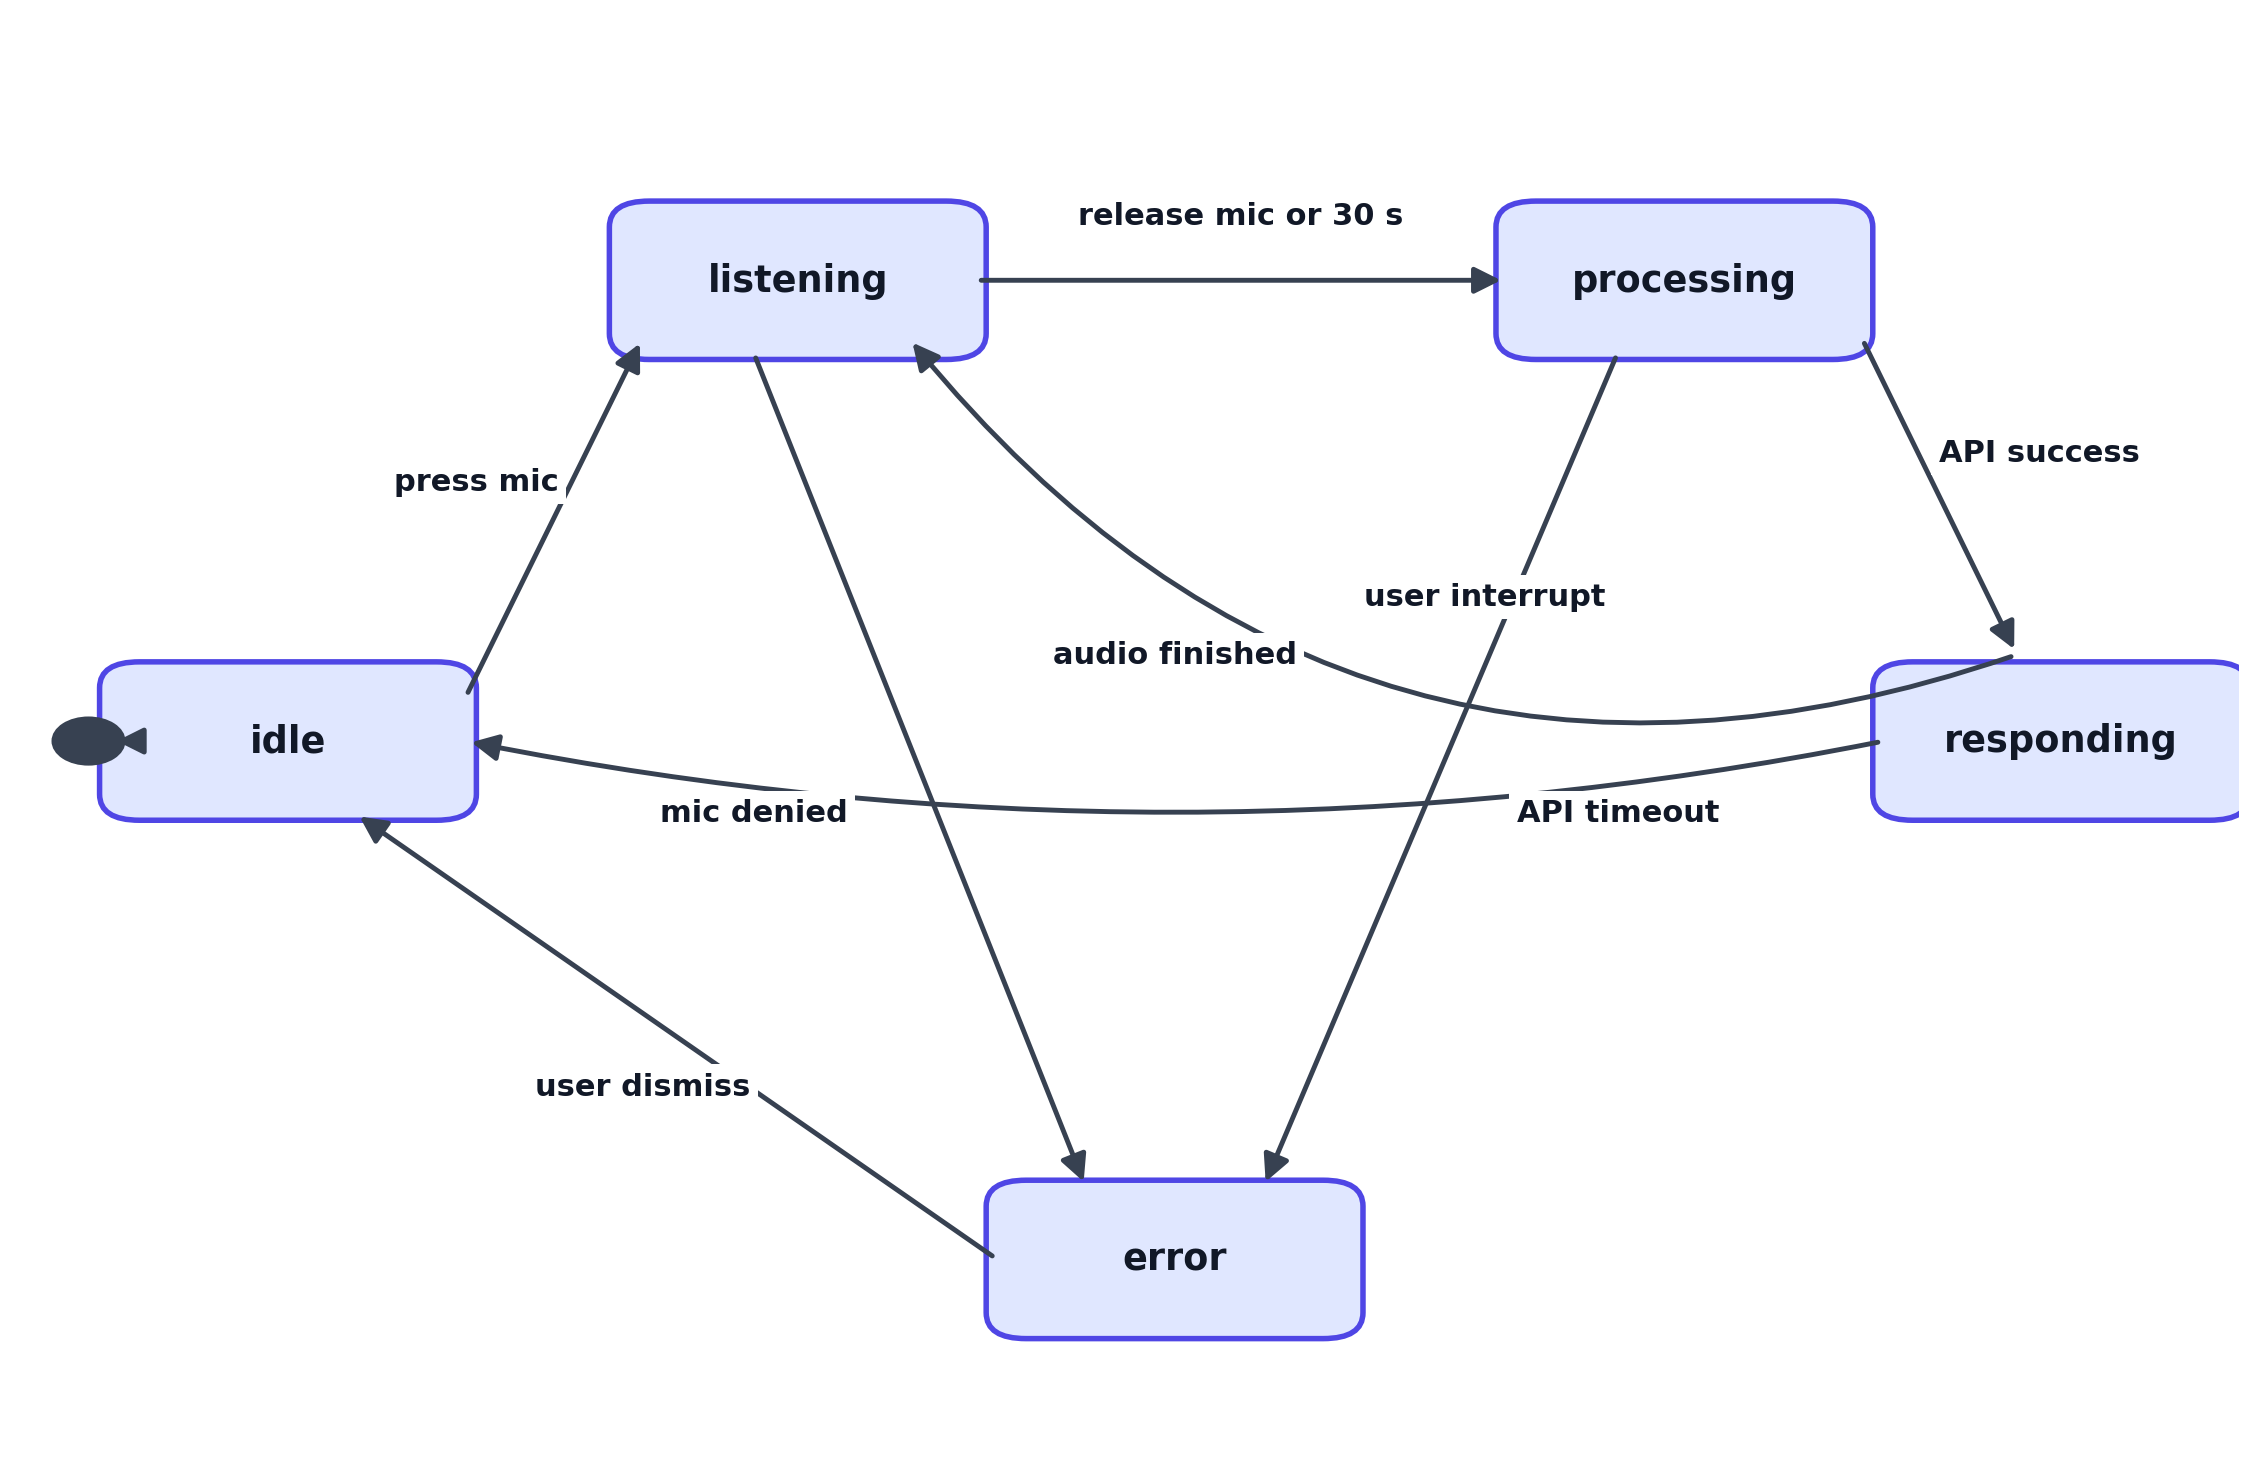
\includegraphics[width=0.7\textwidth]{figures/fig4_state_diagram.png}
  \caption{State diagram of the voice recorder hook.}
  \label{fig:state}
\end{figure}

\subsubsection{Testing}

\begin{table}[H]
  \centering
  \begin{tabular}{p{5cm} p{3cm} p{5cm}}
    \toprule
    \textbf{Test Type}              & \textbf{Result} & \textbf{Notes} \\
    \midrule
    End to end latency              & 4.8 s avg.      & Meets NFR-01 target of under 5 s. \\
    Query accuracy (in scope set)   & 5/5 (100\%)     & All factual claims matched the knowledge base. \\
    Out of scope fallback           & 3/3 (100\%)     & No hallucinated content observed. \\
    Concurrent sessions             & 20 sessions     & No degradation observed. \\
    Idempotent re-upload            & Pass            & Duplicate chunks not created. \\
    Conversation continuity         & Pass            & Follow up queries resolved correctly. \\
    \bottomrule
  \end{tabular}
\end{table}

% ============================================================
% 6. USER MANUAL
% ============================================================
\newpage
\section{User Manual}

\subsection{For Prospective Students and Parents}

\subsubsection{Open the Website}
Navigate to the FAST Peshawar website, or open the direct URL provided
by the admissions office. The application loads inside any modern
browser, including the browser on a mobile phone. There is nothing to
install and no account to create.

\subsubsection{Allow Microphone Access}
When the browser asks for permission, click \textbf{Allow} to grant
microphone access. This permission is needed only for voice queries.
Typed queries do not need it.

\subsubsection{Start the Conversation}
Click the microphone button on the voice card or the circular chat
button at the bottom right corner of the screen. A pulsing animation
shows that the system is listening.

\subsubsection{Speak your Question in Urdu}
Speak clearly. For example: \textbf{FAST Peshawar mein BS ke liye apply
kaise karna hai?} The query is submitted automatically when you finish
speaking, or after the 30 second cap is reached.

\subsubsection{Receive the Answer}
The system shows your question and the assistant's reply as text bubbles
in the chat panel, and reads the reply aloud in Urdu. To stop the audio
early, click the microphone button at any time.

\subsubsection{Ask a Follow-up Question}
You do not need to reset anything. Just keep talking. The system
remembers the last three exchanges and resolves references like
\textit{aur uski fees kitni hai?} against the previous turn. To start
fresh, click the \textbf{New Conversation} button, which clears the
history.

\subsubsection{Continue or End Conversation}
You may keep asking questions for as long as you like. When you are
finished, click the same microphone button to close the session. A full
transcript of the exchange remains visible until the page is closed.

\subsection{For Administrators}

\subsubsection{Open the Admin Panel}
Append \texttt{/admin} to the application URL. Enter the administrator
credentials when the browser prompts for them.

\subsubsection{Review the Knowledge Base}
Once you are signed in, the panel shows a table of all current knowledge
base sources. Each row has a filename and a short description of the
category it covers.

\subsubsection{Upload New Content}
Scroll to the \textit{Add to Knowledge Base} section and drop a
\texttt{.txt} file onto the upload zone, or click the zone to browse for
a file. The file has to be plain text and at most 2 MB. Click
\textit{Upload and Embed} to start ingestion. A spinner is shown while
the file is being processed. Please do not close the tab during this
step.

\subsubsection{Confirm or Retry}
On success, a green confirmation banner appears with the filename of the
ingested document. On failure, a red error banner appears with the
reason. The source table refreshes by itself after a successful upload.

% ============================================================
% 7. CONCLUSIONS AND RECOMMENDATIONS
% ============================================================
\newpage
\section{Conclusions and Recommendations}

\subsection{Conclusions}

Mahir on Call shows that a real time Urdu voice AI system can be built
and deployed for a domain specific use case inside the time and budget of
a Final Year Project. The system meets all the primary objectives we set
out at the start. It supports natural Urdu voice conversation. It
delivers accurate answers from a curated knowledge base. It provides a
live transcript on screen. It includes a moderator escalation route for
queries that fall outside scope. And the average end to end latency is
about 4.8 seconds, comfortably under the five second target.

More importantly, the project is a small proof point for a wider design
idea. Digital inclusion in Pakistan starts with putting spoken Urdu at
the centre of the interface, not as an afterthought. The architecture
shows that the gap between English first AI products and the people they
leave behind is not really a technical wall. It is a question of whose
needs you put first when you design. The retrieval based grounding
mechanism gives us a clean way to keep the model honest, which is what
makes a generative system safe to use in a setting where the wrong
answer can cost a student a year.

\subsection{Recommendations}

\begin{itemize}
  \item \textbf{Annual knowledge base review}:
        The knowledge base should be reviewed and updated by the
        admissions team before every admission season. Fee structures,
        programme offerings, scholarship criteria, and application
        procedures all change, and an outdated answer is more harmful
        than a missing one because the system delivers it with the same
        confidence.
  \item \textbf{Multi-campus rollout}:
        The architecture is intentionally modular. The knowledge base is
        the only campus specific piece. Bringing the same platform up at
        another FAST campus or another Pakistani university needs nothing
        more than a fresh knowledge base and a small number of
        configuration changes.
  \item \textbf{Analytics dashboard}:
        Logging query topics, latency by stage, and a thumbs up or
        thumbs down feedback signal would tell the admissions office
        which questions applicants actually ask most. The same data
        would feed back into the official communication materials and
        into the retrieval thresholds that decide when to fall back.
  \item \textbf{WhatsApp channel}:
        Most of the target audience already lives on WhatsApp. Adding a
        voice note channel through a webhook would extend the system's
        reach without changing the core pipeline, since the backend is
        channel agnostic by design.
\end{itemize}

% =====================  REFERENCES  ==================================
\newpage
\section*{References}
\addcontentsline{toc}{section}{References}

\begin{flushleft}

Brown, T., Mann, B., Ryder, N., Subbiah, M., Kaplan, J., Dhariwal, P.,
Neelakantan, A., Shyam, P., Sastry, G., Askell, A., \& others. (2020).
Language models are few-shot learners. \textit{Advances in Neural
Information Processing Systems}, 33, 1877--1901.

\vspace{0.5em}

Lewis, P., Perez, E., Piktus, A., Petroni, F., Karpukhin, V., Goyal, N.,
K{\"u}ttler, H., Lewis, M., Yih, W.-t., Rockt{\"a}schel, T., \& others.
(2020). Retrieval-augmented generation for knowledge-intensive NLP
tasks. \textit{Advances in Neural Information Processing Systems}, 33,
9459--9474.

\vspace{0.5em}

Radford, A., Kim, J. W., Xu, T., Brockman, G., McLeavey, C., \&
Sutskever, I. (2023). Robust speech recognition via large-scale weak
supervision. In \textit{Proceedings of the 40th International
Conference on Machine Learning} (pp.\ 28492--28518). PMLR.

\vspace{0.5em}

Vaswani, A., Shazeer, N., Parmar, N., Uszkoreit, J., Jones, L.,
Gomez, A. N., Kaiser, {\L}., \& Polosukhin, I. (2017). Attention is all
you need. \textit{Advances in Neural Information Processing Systems},
30.

\vspace{0.5em}

Devlin, J., Chang, M.-W., Lee, K., \& Toutanova, K. (2019). Pre-training
of deep bidirectional transformers for language understanding. In
\textit{Proceedings of NAACL-HLT 2019} (pp.\ 4171--4186). Association
for Computational Linguistics.

\vspace{0.5em}

Robertson, S., \& Zaragoza, H. (2009). The probabilistic relevance
framework: BM25 and beyond. \textit{Foundations and Trends in
Information Retrieval}, 3(4), 333--389.

\vspace{0.5em}

Johnson, J., Douze, M., \& J{\'e}gou, H. (2021). Billion-scale similarity
search with GPUs. \textit{IEEE Transactions on Big Data}, 7(3),
535--547.

\vspace{0.5em}

UNESCO Institute for Statistics. (2023). \textit{Pakistan: literacy
rate, adult total (\% of people ages 15 and above)}. Retrieved from
\url{https://uis.unesco.org/en/country/pk}

\vspace{0.5em}

Government of Pakistan. (2021). \textit{Pakistan Social and Living
Standards Measurement Survey (PSLM) 2019--20}. Pakistan Bureau of
Statistics.

\vspace{0.5em}

Akbar, A. Q., Akhter, M. A., \& Iqbal, A. (2022). Urdu natural language
processing: a comprehensive survey. \textit{IEEE Access}, 10,
55498--55516.

\end{flushleft}

% =====================  APPENDIX  ====================================
\newpage
\appendix
\renewcommand{\thesection}{Appendix \Alph{section}}

\section{Sample Evaluation Queries}
\label{app:queries}

The following table lists a representative sample of evaluation queries
used to measure system accuracy and fallback behaviour. Queries 1 to 5
are in scope. The knowledge base contains authoritative information for
them. Queries 6 to 8 are out of scope, where the system is expected to
deliver a defined fallback response rather than fabricate an answer.

\begin{longtable}{p{1cm} p{8cm} p{4cm}}
  \toprule
  \textbf{No.} & \textbf{Query} & \textbf{Expected Topic} \\
  \midrule
  \endhead
  1  & PhD applicants ke liye minimum requirements kya hain? & Admissions \\
  2  & 2025 ke admission process mein application submission ki dates kya hain? & Admissions \\
  3  & Provisional admission kis ko di ja sakti hai? & Admissions \\
  4  & Admission ke baad candidates ko kaunsi additional support provide ki ja sakti hai? & General Information \\
  5  & Applicants ko kaun se documents submit karne zaroori hain? & Admissions \\
  6  & FAST mein student counseling ya mental health support service available hai? & Out of scope \\
  7  & University ki library digital resources aur e-books ka kitna collection hai? & Out of scope \\
  8  & Kya university apne students ke liye health insurance ya medical coverage plans offer karti hai? & Out of scope \\
  \bottomrule
\end{longtable}

\section{AI Tool Usage Disclosure}
\label{app:ai-disclosure}

In line with the Student's Declaration, the generative AI tools listed
below were used during the preparation of this report and the
associated software. Final responsibility for choosing, applying, and
interpreting any AI assisted material rests with the named authors.

\begin{itemize}
  \item \textbf{Claude} (Anthropic, Inc.) was used for polishing the
        language of written sections of this report, for code review
        and debugging help during backend and frontend development, and
        for the first drafts of the system prompt templates in the
        retrieval module. Every passage that the tool helped with was
        read, fact checked, and substantially rewritten by us before
        going into the final document.
  \item \textbf{GitHub Copilot} (Microsoft Corporation and GitHub,
        Inc.) was used as an in editor code completion assistant during
        frontend development. We accepted, modified, or rejected each
        suggestion as we went.
  \item \textbf{ChatGPT} (OpenAI) was used for early exploratory
        research into available Urdu speech and language tooling, and
        for early drafts of the knowledge base ingestion script. Every
        output was checked against the official documentation before
        being relied on.
\end{itemize}

\end{document}
